%
% Hauptdatei
%


\documentclass[pdftex,a4paper,12pt,DIV15,BCOR20mm,parskip,numbers=noenddot]{scrbook}

	\usepackage{german, ngerman} %Deutsche Trennungen, Anf�hrungsstriche und mehr
	\usepackage[ngerman,german]{babel} % dt. Sprache laden (u.a. auch Ausgabe feststehender Begriffe in deutsch wie etwa Inhaltsverzeichnis statt table of contents)
	\usepackage[latin1]{inputenc} % Zeichenkodierung laden f�r Unix/Windows-Systeme
	\usepackage[babel,german=quotes]{csquotes} % Deutsche Eingabe von �,�,�,� erlauben	
	\usepackage[T1]{fontenc}
  \usepackage[pdftex]{color} 
  \usepackage{setspace} % Das Paket setspace erm�glicht ein einfaches Umstellen von normalem, anderthalbfachen oder doppeltem Zeilenabstand.
  \usepackage{graphics} %Zum Einbinden von Grafiken
  \usepackage[pdftex]{graphicx}  
	\usepackage[final]{listings}  % erm�glicht die Darstellung von (Programm-)Quellcode in der Arbeit
  \usepackage{ae,aecompl}  % ben�tigt zur PDF-Erzeugung, vgl http://dsanta.users.ch/resources/type1.html
  \usepackage[normalem]{ulem} % erm�glicht das Unterstreichen von Text
  \usepackage{amsfonts} % ok-zeichen usw
  \usepackage{scrpage2}
  \usepackage{bibgerm}
  \usepackage{array} % f�r tabellen
  
  \usepackage{times}
  \usepackage{algorithm}
  \usepackage{xspace}
  \usepackage{algpseudocode}
  \usepackage{amsmath}
  
  \usepackage{pgfplots}
  \usepackage{pgfplotstable}
  \pgfplotsset{width=14cm,compat=1.9}
  \usepackage{tikz}
  \usepackage{filecontents}
  
  \usepackage{amsthm}
  \theoremstyle{definition}
  \newtheorem{bsp}{Beispiel}
  
  \usepackage[section]{placeins}
  
  \usepackage{forest}
  \tikzset{el style/.style={midway, font=\scriptsize, inner sep=+1pt, auto=right}}
  \forestset{angled/.style={
  		content/.expanded={\noexpand\textless\forestov{content}\noexpand\textgreater}}}
  
  \newcommand{\Eop}[3][\!]{#2#1\to#1#3}
  \newcommand{\Assign}[2]{\mbox{$#1\leftarrow #2$}}
  \newcommand{\Size}[1]{|#1|}
  \newcommand{\Upto}[0]{\textbf{upto}\xspace}
  \newcommand{\Subchar}[2]{#1[#2]}
  \newcommand{\Substring}[3]{#1[#2\ldots#3]}
  \newcommand{\Rtab}[1][j_{0}]{R_{#1}}
  \newcommand{\EDcol}[1]{E_{\mathsf{col}}^{#1}}
  \newcommand{\Rcol}[1]{\Rtab^{#1}}
  \newcommand{\Deletion}[2][\!]{\Eop[#1]{#2}{\varepsilon}}
  \newcommand{\Insertion}[2][\!]{\Eop[#1]{\varepsilon}{#2}}
  \newcommand{\Replacement}[3][\!]{\Eop[#1]{#2}{#3}}
  \newcommand{\Substitution}[3][\!]{\Eop[#1]{#2}{#3}}
  \newcommand{\Crosspoints}[0]{C}
  \newcommand{\EvalCPname}[0]{\textit{evaluatecrosspoints}}
  \newcommand{\Rounddown}[1]{\left\lfloor#1\right\rfloor}
  \newcommand{\Roundup}[1]{\left\lceil#1\right\rceil}
  \newcommand{\Evalallcolsname}[0]{\mathit{evaluateallcolumns}}
  \newcommand{\Evalallcols}[3]{\Evalallcolsname(E,R,#1,#2,#3)}
  \newcommand{\EvalCP}[4]{\EvalCPname(\Crosspoints,#1,#2,#3,#4)}

	% Beliebige Farben definieren (bei Bedarf auskommentieren und selbst benennen und festlegen)
%	\definecolor{hellblau}{RGB}{238,242,247}
	
	\usepackage{colortbl} % f�r farbige Tabellen
	\usepackage{longtable} % f�r mehrseitige Tabellen
%	\usepackage{booktabs} % f�r tabellen: baut \midrule, \toprule und \bottomrule ein
%	\setlength{\tabcolsep}{30pt} % in Tabellen: Padding des Spalten nach links und rechts
	\renewcommand{\arraystretch}{1.25} % in Tabellen: Padding des Textes nach oben und unten in Prozent

	% Benutzt man bestimmte Spaltendefinitionen (hier: Spaltentyp p mit 25% Breite) �fter, kann man diese hier auslagern und unter einem bestimmten Buchstaben (hier: A) speichern
%	\newcolumntype{A}{p{0.25\textwidth}} 

	\usepackage{nomencl} % Package f�r ein Abk�rzungsverzeichnis
	\renewcommand{\nomname}{Abk�rzungsverzeichnis} % Deutsche �berschrift
	\setlength{\nomlabelwidth}{.20\hsize} % Breite eines Eintrags
	\renewcommand{\nomlabel}[1]{#1 \dotfill} % Auff�llen mit Punkten
	\setlength{\nomitemsep}{-2\parsep} % Zeilenabstand verkleinern
	\makenomenclature  % Datenbank des Abk�rzungsverzeichnisses beim Kompilieren des Textes erzeugen

	% fuer Literaturverweise
	\usepackage[numbers,square]{natbib}
	\bibpunct{[}{]}{;}{a}{}{;} % Natbib konfigurieren, so da� im text [M�ller 2006] erscheint und keine runden Klammern o.�.
	\renewcommand{\cite}{\citep} % \cite zu \citep umwandeln, so dass im Text \cite{Mueller.2006} f�r Referenzen verwendet werden kann.
%	\usepackage{url} % damit im LitVZ auch so etwas wie 'M�ller 2006: Vortrag zum Thema XY (Powerpoint-Pr�sentation)' steht; (Dateiendungen werden also textuell repr�sentiert)

	%% Verhindert, dass im Literaturverzeichnis nach der Nennung von [Mueller 2006] die Seite umgebrochen wird und die Autoren + Buchtitel etc. auf der n�chsten Seite landen
	%% Es wurde daher \noparagraphbreak in der natdin.bst bei der Ausgabe der Elemente erg�nzt
	%% siehe http://groups.google.de/group/de.comp.text.tex/browse_thread/thread/9ca4c681e2063fbd/f7eb3eec044b058e
	\makeatletter
	\def\noparagraphbreak{\interlinepenalty10000
	  \@itempenalty-\@highpenalty}
	\makeatother 


	% Fu�noten werden im gesamten Dokument fortlaufend hochgez�hlt und nicht nur kapitelweise, vgl. http://www.golatex.de/nummerierung-der-fussnoten-durchgehend-im-gesamten-dokument-t2042.html
	\usepackage{chngcntr}
	\counterwithout{footnote}{chapter}

	\setlength{\emergencystretch}{1em} % F�r den Fall, dass Zeilen im 1. Anlauf nicht richtig umgebrochen werden k�nnen, einen 'Notfallraum' einrichten (vgl. http://www.golatex.de/overfull-boxes-in-latex-t1979.html) 

	% Definitionen werden mit Hilfe von 'dfn' eingeleitet und k�nnen somit zentral formatiert werden.
	\newtheorem{dfn}{Definition}
	
	% entnommen aus http://www.siart.de/typografie/latextipps.xhtml#floats
	\renewcommand{\floatpagefraction}{0.8} % gibt den Bruchteil einer Seite, die f�r Gleitobjekte benutzt wird, an, der erreicht werden muss, bevor eine neue Seite angefangen wird. (Standard: 0.5; d.h. wenn ein Bild 51% der Seite einnimmt, wird extra f�r dieses Bild eine ganze Seite reserviert --> unsch�n)
	\renewcommand{\topfraction}      {0.8}
	\renewcommand{\bottomfraction}   {0.5} % \topfraction / \bottomfraction, gibt den Bruchteil einer Seite an, bis zu dem Gleitobjekte oben bzw. unten angeordnet werden sollen.
	\renewcommand{\textfraction}     {0.15} % gibt den Bruchteil einer Seite an, der mit Text belegt werden k�nnen muss.
	\makeatletter
	  \setlength{\@fptop}{0pt} % Wenn ein Float-Objekt allein auf einer Seite steht, soll es am oberen Rand der Seite erscheinen und nicht vertikal zentriert
	\makeatother
	
	% schrift auf palatino umstellen
  \usepackage{palatino}
  \setkomafont{sectioning}{\normalcolor\bfseries}


	% PDF-Support einbinden und konfigurieren
  \usepackage[
  	pdfstartview={Fit},   
  	pdffitwindow=true,
  	colorlinks,
  	linkcolor=black,
  	anchorcolor=black,
  	citecolor=black,
  	urlcolor=black
  ]{hyperref}
  \hypersetup
  {
  	pdftitle     = {Diplomarbeit zum Thema XY},
  	pdfsubject   = {Universit�t Hamburg / Department Informatik / ITG / Diplomarbeit},
  	pdfauthor    = {Vorname Nachname},
  	pdfkeywords  = {Diplomarbeit, Universit�t Hamburg}, % Hier kann eine beliebige Liste von Schl�sselw�rtern eingegeben werden, die z.B. Windows zur Indexierung/Suche benutzt
  	plainpages   = false 
  }
 
   
  % Zeilenabstand
  \setstretch{1.24}   

	% Strafpunkte, die beim Seitenumbruch vergeben werden, falls die erste Zeile eines Absatzes allein auf der vorangehenden Seite verbleibt. vgl http://www.jr-x.de/publikationen/latex/tipps/zeilenumbruch.html
	\clubpenalty=150

	% Strafpunkte, die beim Seitenumbruch vergeben werden, falls die letzte Zeile gerade noch auf die n�chste Seite umgebrochen wird. vgl http://www.jr-x.de/publikationen/latex/tipps/zeilenumbruch.html
	\widowpenalty=150  

  % Pagestyle definieren (nach Martins Template)
	\defpagestyle{diplHeadings}
	{ % es folgt: Definition des Seitenkopfes: 
	  % obere Linie
		(0pt,0pt)
		% linke Seite
		{\upshape \rlap{\pagemark} \hfill \headmark \hfill} % auf einer linken Seite soll LINKS die Seitenzahl stehen und mittig die Headline (headmark)
		% rechte Seite
		{\upshape \hfill \headmark \hfill \llap{\pagemark}} % auf einer rechten Seite soll RECHTS die Seitenzahl stehen und mittig die Headline (headmark)
		% falls Layout "one page"
		{}
		% untere Line
		(\textwidth,1pt)
	}
	{ % es folgt: Definition des Seitenfu�es: Wir wollen lediglich eine schwarze, �ber die komplette Seite gehende Linie erzeugen
	  % obere Linie
		(\textwidth,1pt)
		% linke Seite
		{}
		% rechte Seite
		{}
		% falls Layout "one page"
		{}
		% untere Linie
		(0pt,0pt)
	}  
	% Pagestyle auch f�r Chapter-Anfang einrichten
	\renewcommand*{\chapterpagestyle}{diplHeadings}
	\renewcommand*{\chapterheadstartvskip}{\vspace*{-\topskip}}
	\automark[section]{chapter}


	% R�nder	
	\setlength{\textwidth}{15cm}        % Textbreite
	\setlength{\textheight}{24cm}       % Texth�he
	\setlength{\topmargin}{-12mm}       % oberer Rand
  
 
  % Listingsformatierung (Quelltexte)
  \definecolor{lightgrey}{rgb}{0.90,0.90,0.90}
  \lstloadlanguages{XML}
  \lstset{
    tabsize=2,
    escapeinside={(*@}{@*)},
    captionpos=t,
    framerule=0pt,
    backgroundcolor=\color{lightgrey},
    basicstyle=\small\ttfamily,
    keywordstyle=\small\bfseries,
    numbers=left,
    fontadjust
  }    
%
% EOF
%  % Einbinden der Konfigurationen

\begin{document}


%
% Titelseiten Datei
%

\begin{titlepage}

	% Fehler "destination with the same identifier" unterdr�cken...
  \setcounter{page}{-1}

	% Titelseite
	\begin{figure}[h]
		\begin{minipage}[b]{25mm}
			
\includegraphics[width=25mm,clip]{images/logo_uhh}
		\end{minipage}
		\begin{minipage}[b]{2mm}
			
\includegraphics[width=1mm,height=24mm]{images/greypixel}
		\end{minipage}
		\begin{minipage}[b]{12 cm}
			{\sffamily
				{\Large Universit�t Hamburg } \\
				Fakult�t f�r Mathematik,\\
				Informatik und Naturwissenschaften \\
				Department Informatik \\
			}
		\end{minipage}
	\end{figure}

	\vfill
	
	\begin{center}
		% Diplomarbeit 
		\noindent { \huge
			Bachelorarbeit \\
					}
		\vspace{14mm}
		% Titel
		\noindent \textbf{\Large
		  Speichereffiziente Methoden zur Repr�sentation \\
		  von paarweisen Sequenz-Alignments \\		  
		}
		\vspace{10mm}
		
		%\noindent {\large
		%(Option:) In Kooperation mit:
		
		%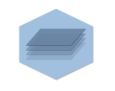
\includegraphics{images/logoitg.png}\\ %Firmenlogo
		%<Firma> \\
		%<Bereich / Abteilung>
		%}
	\end{center}
	
	\vfill
	
	\noindent \textbf{Thorben Wiese} \\
	\noindent \rule{\textwidth}{0.4mm} 
	\noindent{\textrm{3wiese@informatik.uni-hamburg.de}} \\
	\noindent{\textrm{Studiengang B.Sc. Informatik}} \\
	\noindent{\textrm{Matr.-Nr. 6537204}} \\
	\noindent{\textrm{Fachsemester 6}} \\
	\begin{tabbing}
	\hspace{20em} \=  \kill
	Erstgutachter Universit�t Hamburg: \> Prof. Dr. Stefan Kurtz \\
	Zweitgutachter Universit�t Hamburg: \> Dr. Giorgio Gonnella \\
		
	\hspace{20em} \=  \kill
	
	%(Option)Betreuer <Firma>: \> <Vorname> <Name> \\
			
	\end{tabbing}
	
	% R�ckseite der Titelseite mit Zitat
	\newpage 
	\thispagestyle{empty}
	\setcounter{page}{0}

	% wenn man Lust auf ein Zitat hat...
	% ... ansonsten auskommentieren
	~\\ \vfill \noindent 
%	A distributed system is one where the failure of some \\
%	computer I've never heard of can keep me from getting my work done. \\
%	\textit{-- Leslie Lamport}
\end{titlepage}

%
% EOF
%

% pagestyle umschalten
\pagestyle{diplHeadings}

\nomenclature{IT}{Informationstechnik}
\nomenclature{WWW}{World Wide Web} % Einbinden der zentralen Datei, die alle Abk�rzungen enth�lt
%
% Inhaltsverzeichnis
%

% --> Seitennummerierung r�misch
\pagenumbering{Roman}
\setcounter{page}{1}
\pdfbookmark[1]{Inhaltsverzeichnis}{toc}

\tableofcontents
%\cleardoublepage

%
% Abbildungs- und Tabellenverzeichnis
%
\listoffigures
\listoftables
%\cleardoublepage

%
% Abk�rzungsverzeichnis ausgeben
%
%\markboth{Abk�rzungsverzeichnis}{Abk�rzungsverzeichnis} % Kopfzeile anpassen, vgl. http://www.golatex.de/falsche-kopfzeile-im-abkuerzungsverzeichnis-t2074.html
%\printnomenclature % Abk�rzungsverzeichnis
%\cleardoublepage
%
% EOF
% % Inhalts-, Abbildungs-, Tabellenverzeichnis und Abk�rzungsverzeichnis laden (und ausgeben)

% KAPITEL
% --> Seitennummerierung wieder arabisch
\pagenumbering{arabic}
\setcounter{page}{1}
%%
% Einleitung
%

\chapter{Aufbau}


\begin{enumerate}
	\item Einleitung
	\begin{itemize}
		\item Problem darstellen
	\end{itemize}
	\item CIGAR
	\begin{itemize}
		\item Komplexit�t
		\item Speicherverbrauch
		\item Grafiken
	\end{itemize}
	\item TracePoint Konzept
	\begin{itemize}
		\item Komplexit�t
		\item Speicherverbrauch
		\item Grafiken
	\end{itemize}
	\item Optimierung
	\begin{itemize}
		\item Delta Encoding
		\item Grafiken Vergleich
	\end{itemize}
	\item Code
	\begin{itemize}
		\item UML Aufbau
		\item Funktionen erkl�ren
	\end{itemize}
	\item Fazit
	\begin{itemize}
		\item Problem durch Programm gel�st
	\end{itemize}
\end{enumerate}

%
% Einleitung
%

\chapter{Einleitung}

Ein Sequenzalignment wird in der Bioinformatik dazu verwendet, zwei oder mehrere Sequenzen von zum Beispiel DNA-Str�ngen oder Proteinsequenzen miteinander zu vergleichen und die Verwandtschaft zu bestimmen. Ein Alignment ist das Ergebnis eines solchen Vergleichs. Bei einem globalen Alignment wird jeweils die gesamte Sequenz betrachtet, bei einem lokalen Alignment lediglich Teilabschnitte der beiden Sequenzen.
Um die verschiedenen Sequenzen vergleichen zu k�nnen, berechnet man einen Score oder die Kosten, um den Aufwand, den man betreiben muss, um die gegebenene Sequenz in die Zielsequenz umzuwandeln, beschreiben zu k�nnen. Hierbei wird jeweils das Optimum, also entweder der maximale Score oder die minimalen Kosten gesucht.
Die verschiedenen Schritte, um die Symbole der Strings zu ver�ndern, sind bei Gleichheit ein 'match', bei der Substitution ein 'mismatch', bei der L�schung eine 'deletion' und bei der Einf�gung eine 'insertion', welche je nach Verfahren unterschiedlich gewichtet werden k�nnen. Hierbei haben �hnliche Sequenzen einen hohen Score und geringe Kosten und unterschiedliche Sequenzen analog einen kleinen Score und hohe Kosten.

\section*{Die Edit-Operationen}

Die hier eingef�hrten Begriffe werden in \cite[S. 5-7, 14-16]{gsa-skript} definiert.

Sei $\mathcal{A}$ eine endliche Menge von Buchstaben, die man Alphabet nennt. F�r DNA-Sequenzen verwendet man �blicherweise die Menge der Basen, also $\mathcal{A} = \{a, c, g, t\}$. $\mathcal{A}^i$ sei die Menge der Sequenzen der L�nge $i$ aus $\mathcal{A}$ und $\varepsilon$ sei die leere Sequenz. Formal ausgedr�ckt ist eine Edit-Operation ein Tupel 
\[(\alpha, \beta) \in (\mathcal{A}^1 \cup \{\varepsilon\}) \times (\mathcal{A}^1 \cup \{\varepsilon\}) \backslash \{(\varepsilon, \varepsilon)\},\]

Eine �quivalente Schreibweise von $(\alpha,\beta)$ ist $\alpha \rightarrow \beta$. Es gibt drei verschiedene Edit-Operationen
\begin{align*}
a \rightarrow \varepsilon &\indent \text{ ist eine Deletion f�r alle }a \in \mathcal{A}\\
\varepsilon \rightarrow b &\indent \text{ ist eine Insertion f�r alle }b \in \mathcal{A}\\
a \rightarrow b &\indent \text{ ist eine Substitution f�r alle }a,b \in \mathcal{A}
\end{align*}
Dabei ist zu beachten, dass $\varepsilon \rightarrow \varepsilon$ keine Edit-Operation darstellt.

Ein Alignment von zwei Sequenzen $u$ und $v$ l�sst sich nun als eine Sequenz $(\alpha_1 \rightarrow \beta_1, ... , \alpha_h \rightarrow \beta_h)$ von Edit-Operationen definieren, sodass $u = \alpha_1 ... \alpha_h$ und $v = \beta_1 ... \beta_h$ gilt.

\section*{Die Edit-Distanz}

Sei eine Kostenfunktion $\delta$ mit $\delta(a\rightarrow b)\geq 0$ f�r alle Substitutionen $a \rightarrow b$ und $\delta(\alpha \rightarrow \beta)>0$ f�r alle Einf�gungen und L�schungen $\alpha \rightarrow \beta$ gegeben. Die Kosten f�r ein Alignment $A = (\alpha_1 \rightarrow \beta_1, ... , \alpha_h \rightarrow \beta_h)$ ist die Summe der Kosten aller Edit-Operationen des Alignments.
\[\delta(A) = \sum_{i=1}^{h}\delta(\alpha_i \rightarrow \beta_i)\]
Ein Beispiel einer Kostenfunktion ist die Einheitskostenfunktion
\[
\delta(\alpha \rightarrow \beta) = 
\begin{cases} 
0 ,& \text{wenn } \alpha,\beta \in \mathcal{A} \text{ und } \alpha=\beta \\
1 , & \text{sonst.}
\end{cases}
\]
Die Edit-Distanz von zwei Sequenzen ist wie folgt definiert:
\[edist_\delta(u,v) = \min\{\delta(A) \mid A \text{ ist Alignment von }u \text{ und }v\}\]
Ein Alignment A ist optimal, wenn $\delta(A) = edist_\delta(u,v)$ gilt.\\[0,5cm]
Wenn $\delta$ die Einheitskostenfunktion ist, so ist $edist_\delta(u,v)$ die Levenshtein Distanz \cite[S. 19-21]{gsa-skript}.

Ein Alignment kann f�r eine Edit-Distanz $e$ mit der Einheitskostenfunktion in $O(e)$ Zeit berechnet werden \cite[S. 41-42]{gsa-skript}.
%
% Einleitung
%

\chapter{CIGAR-Strings}

Ein Dateiformat, welches zur Speicherung von Alignments verwendet wird, ist das SAM-Format oder die komprimierte Version BAM. Dieses codiert ein Alignment in einem sogenannten Cigar-String der aus einzelnen Zeichen besteht, die jeweil eine Edit-Operation bezeichnen, also M f�r eine Substitution, I f�r eine Insertion und D f�r eine Deletion. Gleiche aufeinanderfolgende Operationen werden als Kombination von Quantit�t und Symbol geschrieben.

Beispiel 1: Sei $u =$ \texttt{actgaact}, $v =$ \texttt{actagaat} und das Alignment $A = (a\rightarrow a, c\rightarrow c, t\rightarrow t, ...)$ gegeben.
\begin{center}
	\texttt{
		\begin{tabular}{ccccccccc}
			a & c & t & - & g & a & a & c & t\\
			$|$&$|$&$|$&&$|$&$|$&$|$& &$|$\\
			a&c&t&a&g&a&a& - &t
		\end{tabular}
	}
\end{center}
Ein Alignment wird �blicherweise in drei Zeilen geschrieben, wobei in der ersten Zeile die Sequenz $u$ und in der dritten Zeile die Sequenz $v$ geschrieben wird. In der mittleren Zeile symbolisiert das Zeichen '$|$' eine Substitution, wobei �blicherweise nur ein Match markiert wird. Au�erdem wird ein $\varepsilon$ aus der Edit-Operation in diesem Fall durch das Zeichen '-' dargestellt.

Dieses Alignment wird duch den Cigar-String \texttt{3M1I3M1D1M} repr�sentiert. Das Format ben�tigt wenig Speicher f�r Alignments mit einer kleinen Edit-Distanz und deutlich mehr Speicher f�r Alignments mit einer gro�en Edit-Distanz \cite{sam}.

\subsection{Komplexit�t}
\clearpage

\subsection{Speicherverbrauch}\label{Cigar_Speicher}
Sei das Alignment $\cal{A}$
\begin{verbatim}
0    5    0    5    0    5    0    5    0    
gagc-a-t-gttgcc-tggtcctttgctaggtactgta-gaga
|| | | | |  | | ||| |||| ||| ||| ||||| ||||
gaccaagtag--g-cgtggacctt-gctcggt-ctgtaagaga
0    5    0    5    0    5    0    5    0   
\end{verbatim}
und der dazugeh�rige CIGAR-String \texttt{4M1D1M1D1M1D1M2I1M1I1M1D8M1I7M1I5M1D4M} gegeben.

Mit einer naiven bin�ren Kodierung br�uchte man demnach f�r jedes Symbol $c \in \cal{A}$ $log_2(38) = 6$ Bit pro Symbol, also $38 \cdot 6 = 228$ Bit insgesamt.

Bei einer \textit{minimalen} bin�ren Kodierung, wie sie auch im Huffman-Alogrithmus verwendet wird, werden die L�ngen der Codew�rter anhand der relativen Wahrscheinlichkeit des Symbols im Alphabet angepasst. Somit l�sst sich eine Kodierung erm�glichen, welche im Durchschnitt weniger Bits pro Symbol beansprucht \cite{coding}.

Der Huffman-Algorithmus w�rde bei dem oben genannten Beispiel der TracePoints wie folgt ablaufen:

Gegeben sei das Alphabet $\cal{A}$ $= \{M, I, D, 1, 2, 4, 5, 7, 8\}$, sowie die relativen Wahrscheinlichkeiten $p(i)$ jeden Symbols aus $\cal{A}$ mit

\begin{tabular}{lcl}
$p(1)$&=& $\frac{13}{38}$\\
$p(M)$ &=& $\frac{10}{38}$\\
$p(D)$ &=& $\frac{5}{38}$\\
$p(I)$ &=& $\frac{4}{38}$\\
$p(4)$ &=& $\frac{2}{38}$\\
$p(2)$ &=& $\frac{1}{38}$\\
$p(5)$ &=& $\frac{1}{38}$\\
$p(7)$ &=& $\frac{1}{38}$\\
$p(8)$ &=& $\frac{1}{38}$
\end{tabular}

Ausf�hrung des Huffman-Algorithmus:

\begin{tabular}{llc}
	$\frac{13}{38}$ & $c_1 = \lambda$&\\
	$\frac{10}{38}$ & $c_2 = \lambda$&\\
	$\frac{5}{38}$ & $c_3 = \lambda$&\\
	$\frac{4}{38}$ & $c_4 = \lambda$&$\Rightarrow$\\
	$\frac{2}{38}$ & $c_5 = \lambda$&\\
	$\frac{1}{38}$ & $c_6 = \lambda$&\\
	$\frac{1}{38}$ & $c_7 = \lambda$&\\
	$\frac{1}{38}$ & $c_8 = \lambda$&\\
	$\frac{1}{38}$ & $c_9 = \lambda$&
\end{tabular}\begin{tabular}{llc}
	$\frac{13}{38}$ & $c_1 = \lambda$&\\
	$\frac{10}{38}$ & $c_2 = \lambda$&\\
	$\frac{5}{38}$ & $c_3 = \lambda$&\\
	$\frac{4}{38}$ & $c_4 = \lambda$&$\Rightarrow$\\
	$\frac{2}{38}$ & $c_5 = \lambda$&\\
	$\frac{2}{38}$ & $c_6 = 0, c_7 = 1$&\\
	$\frac{1}{38}$ & $c_8 = \lambda$&\\
	$\frac{1}{38}$ & $c_9 = \lambda$&\\
	&&
\end{tabular}\begin{tabular}{llc}
	$\frac{13}{38}$ & $c_1 = \lambda$&\\
	$\frac{10}{38}$ & $c_2 = \lambda$&\\
	$\frac{5}{38}$ & $c_3 = \lambda$&\\
	$\frac{4}{38}$ & $c_4 = \lambda$&$\Rightarrow$\\
	$\frac{2}{38}$ & $c_5 = \lambda$&\\
	$\frac{2}{38}$ & $c_6 = 0, c_7 = 1$&\\
	$\frac{2}{38}$ & $c_8 = 0, c_9 = 1$&\\
	&&\\
	&&
\end{tabular}\begin{tabular}{llc}
	$\frac{13}{38}$ & $c_1 = \lambda$&\\
	$\frac{10}{38}$ & $c_2 = \lambda$&\\
	$\frac{5}{38}$ & $c_3 = \lambda$&\\
	$\frac{4}{38}$ & $c_4 = \lambda$&$\Rightarrow$\\
	$\frac{4}{38}$ & $c_5 = 0, c_6 = 10,$&\\
	&$c_7 = 11$&\\
	$\frac{2}{38}$ & $c_8 = 0, c_9 = 1$&\\
	&&\\
	&&
\end{tabular}

\begin{tabular}{llc}
	$\frac{13}{38}$ & $c_1 = \lambda$&\\
	$\frac{10}{38}$ & $c_2 = \lambda$&\\
	$\frac{5}{38}$ & $c_3 = \lambda$&$\Rightarrow$\\
	$\frac{4}{38}$ & $c_4 = \lambda$&\\
	$\frac{4}{38}$ & $c_5 = 0, c_6 = 10, c_7 = 11$&\\
	$\frac{2}{38}$ & $c_8 = 0, c_9 = 1$&\\
	&&\\
	&&\\
	&&
\end{tabular}\begin{tabular}{llc}
	$\frac{13}{38}$ & $c_1 = \lambda$&\\
	$\frac{10}{38}$ & $c_2 = \lambda$&\\
	$\frac{6}{38}$ & $c_4 = 0, c_8 = 10, c_9 = 11$&$\Rightarrow$\\
	$\frac{5}{38}$ & $c_3 = \lambda$&\\
	$\frac{4}{38}$ & $c_5 = 0, c_6 = 10, c_7 = 11$&\\
	&&\\
	&&\\
	&&\\
	&&
\end{tabular}

\begin{tabular}{llc}
	$\frac{13}{38}$ & $c_1 = \lambda$&\\
	$\frac{10}{38}$ & $c_2 = \lambda$&\\
	$\frac{9}{38}$ & $c_3 = 0, c_5 = 10, c_6 = 110, c_7 = 111$&$\Rightarrow$\\
	$\frac{6}{38}$ & $c_4 = 0, c_8 = 10, c_9 = 11$&
\end{tabular}\begin{tabular}{llc}
	$\frac{15}{38}$ & $c_3 = 00, c_5 = 010, c_6 = 0110, c_7 = 0111,$&\\
	& $c_4 = 10, c_8 = 110, c_9 = 111$&\\
	$\frac{13}{38}$ & $c_1 = \lambda$&\\
	$\frac{10}{38}$ & $c_2 = \lambda$&$\Rightarrow$\\
	&&
\end{tabular}

\begin{tabular}{llc}
	$\frac{23}{38}$ & $c_1 = 0, c_2 = 1$&\\
	$\frac{15}{38}$ & $c_3 = 00, c_5 = 010, c_6 = 0110, c_7 = 0111,$&$\Rightarrow$\\
	& $c_4 = 10, c_8 = 110, c_9 = 111$&\\
	&&\\
	&&
\end{tabular}\begin{tabular}{ll}
$\frac{38}{38}$ & $c_1 = 00, c_2 = 01, c_3 = 100,  c_4 = 110,$\\
 &$c_5 = 1010, c_6 = 10110, c_7 = 10111,$\\
 &$c_8 = 1110, c_9 = 1111$\\
&\\
&
\end{tabular}

Somit ergibt sich die Menge $C$ der Codew�rter mit
\[C = "00", "01", "100", "110", "1010", "10110", "10111", "1110", "1111"\]
und der dazugeh�rige Huffman-Baum:

\begin{center}
\begin{forest}
	for tree={grow'=south}
	[$\frac{38}{38}$
	[$\frac{15}{38}$, edge label={node[midway,right,font=\scriptsize]{1}}
	[$\frac{6}{38}$, edge label={node[midway,right,font=\scriptsize]{1}}
	[$\frac{2}{38}$, edge label={node[midway,right,font=\scriptsize]{1}}
	[$c_9$, edge label={node[midway,right,font=\scriptsize]{1}}]
	[$c_8$, edge label={node[midway,left,font=\scriptsize]{0}}] ]
	[$c_4$, edge label={node[midway,left,font=\scriptsize]{0}}] ]
	[$\frac{9}{38}$, edge label={node[midway,left,font=\scriptsize]{0}}
	[$\frac{4}{38}$, edge label={node[midway,right,font=\scriptsize]{1}}
	[$\frac{2}{38}$, edge label={node[midway,right,font=\scriptsize]{1}}
	[$c_7$, edge label={node[midway,right,font=\scriptsize]{1}}]
	[$c_6$, edge label={node[midway,left,font=\scriptsize]{0}}] ]
	[$c_5$, edge label={node[midway,left,font=\scriptsize]{0}}] ]
	[$c_3$, edge label={node[midway,left,font=\scriptsize]{0}}] ] ]
	[$\frac{23}{38}$, edge label={node[midway,left,font=\scriptsize]{0}} 
	[$c_2$, edge label={node[midway,right,font=\scriptsize]{1}}]
	[$c_1$, edge label={node[midway,left,font=\scriptsize]{0}}] ]
	]
\end{forest}
\end{center}

Der gesamte Bitverbrauch dieser Kodierung ist demnach 32 Bit.

Der durchschnittliche Bitverbrauch f�r ein Symbol betr�gt 
\[\frac{38}{38} + \frac{23}{38} + \frac{15}{38} + \frac{9}{38} + \frac{6}{38} + \frac{4}{38} + \frac{2}{38} + \frac{2}{38} \approx 2.61 \text{ Bit.}\]

Die Entropie betr�gt

\begin{tabular}{lcl}
	$H(X)$ &=& $-(\frac{13}{38} \cdot log_2(\frac{13}{38}) + \frac{10}{38} \cdot log_2(\frac{10}{38}) + \frac{5}{38} \cdot log_2(\frac{5}{38}) + $\\
	&&$\frac{4}{38} \cdot log_2(\frac{4}{38}) + \frac{2}{38} \cdot log_2(\frac{2}{38}) + \frac{1}{38} \cdot log_2(\frac{1}{38}) + $\\
	&&$\frac{1}{38} \cdot log_2(\frac{1}{38}) + \frac{1}{38} \cdot log_2(\frac{1}{38}) + \frac{1}{38} \cdot log_2(\frac{1}{38}))$\\
	&$\approx$& $2.72 \text{ Bit je Symbol}$
\end{tabular}

\subsection{Grafiken}
%
% Einleitung
%

\chapter{TracePoint Konzept}

Ein neuer Ansatz der speichereffizienten Repr�sentation von Alignments wurde von Gene Myers in \cite{myers} beschrieben und basiert auf dem Konzept der Trace Points.

Sei $A$ ein Alignment von $u[i...j]$ und $v[k...\ell]$ mit $i < j$ und $k < l$ und sei $\Delta \in \mathbb{N}$. Sei $p = \left \lceil\frac{i}{\Delta}\right \rceil$. Man unterteilt $u[i...j]$ in $\tau = \left \lceil\frac{j}{\Delta}\right \rceil - \left \lfloor\frac{i}{\Delta}\right \rfloor$ Substrings $u_0, u_1, ... , u_{\tau -1}$ mit
\[  
u_q =
\begin{cases} 
u[i...p\cdot\Delta] & \text{falls }q = 0 \\
u[(p+q-1)\cdot\Delta+1...(p+q)\cdot\Delta] & \text{falls }0<q<\tau -1\\
u[(p+\tau-2)\cdot\Delta...j] & \text{falls }q = \tau -1
\end{cases}
\]

F�r alle $q$ mit $ 0 \leq q < \tau -1$ sei $t_q$ der letzte Index des Substrings von $v$, der in A mit $u_q$ aligniert. $t_q$ nennt man Trace Point. F�r $q = 0$ aligniert $u_0$ mit $v_0 = v[k...t_0]$. F�r alle $q$ mit $0<q< \tau -1$ aligniert $u_q$ mit $v_q = v[t_{q-1}+1...t_q]$.

Seien $i,j,k,\ell,\Delta$ und die Trace-Points eines Alignments von $u$ und $v$ gegeben. Dann kann ein Alignment $A'$ von $u$ und $v$ mit $\delta (A') \leq \delta (A)$ konstruiert werden. Danach bestimmt man aus den Trace-Points die Substring-Paare $u_q$ und $v_q$, berechnet hierf�r ein optimales Alignment und konkateniert die Alignments von den aufeinanderfolgenden Substring-Paaren zu $A'$.

Beispiel 2:
\begin{verbatim}
Sequenz 1: gagcatgttgcctggtcctttgctaggtactgtagaga
Sequenz 2: gaccaagtaggcgtggaccttgctcggtctgtaagaga
Delta: 15

Gesamtalignment:

0    5    0    5    0    5    0    5    0    
gagc-a-t-gttgcc-tggtcctttgctaggtactgta-gaga
|| | | | |  | | ||| |||| ||| ||| ||||| ||||
gaccaagtag--g-cgtggacctt-gctcggt-ctgtaagaga
0    5    0    5    0    5    0    5    0    



seq1[0...14] aligniert mit seq2[0...15]
gagc-a-t-gttgcc-tgg
|| | | | |  | | |||
gaccaagtag--g-cgtgg

seq1[15...29] aligniert mit seq2[16...28]
tcctttgctaggtac
 |||| ||| ||| |
acctt-gctcggt-c

seq1[30...37] aligniert mit seq2[29...37]
tgta-gaga
|||| ||||
tgtaagaga

Trace Points: [15, 28] 
\end{verbatim}

\section{Komplexit�t}

%TODO ausf�hrlicher
 F�r die Trace-Point Repr�sentation wird f�r eine Edit-Distanz $e$ mit Einheitskosten als Kostenfunktion $\delta$ wie oben beschrieben lediglich $O(e^2)$ Zeit pro Teilalignment ben�tigt, wobei bei einer erwarteten Fehlerrate $\varepsilon$ des Alignments die Edit-Distanz immer h�chstens so gro� ist wie die Anzahl der Fehler im Teilalignment. \cite[S.41-42]{gsa-skript}
 
\section{Speicherverbrauch}

\subsection{Delta-Kodierung}\label{Delta-Kodierung}

%TODO

\subsection{Beispiel}
Sei $\Delta = 5$ und das Alignment $A$
\begin{verbatim}
		0    5    0    5    0    5    0    5    0    
		gagc-a-t-gttgcc-tggtcctttgctaggtactgta-gaga
		|| | | | |  | | ||| |||| ||| ||| ||||| ||||
		gaccaagtag--g-cgtggacctt-gctcggt-ctgtaagaga
		0    5    0    5    0    5    0    5    0   
\end{verbatim}

wie in Abschnitt \ref{Cigar_Speicher} mit den dazugeh�rigen TracePoints $5, 10, 15, 20, 24, 28$ und $34$ gegeben. Es ergibt sich somit das Alphabet $\cal{A}$ $= \{5, 10, 15, 20, 24, 28, 34\}$ mit ausschlie�lich positiven und aufsteigenden Werten.

F�r die Trace Points ist somit eine Delta-Kodierung m�glich. Als neue Liste zu kodierender Werte ergibt sich somit nach \ref{Delta-Kodierung} $L = (5, 5, 5, 4, 4, 6)$.

%TODO

Bei der naiven bin�ren Kodierung

F�r die un�re Kodierung

Die Huffman-Kodierung ergibt



%TODO bin�r / un�r / huffman f�r Delta-Kodierung


\subsection{Testl�ufe}

Die folgenden Grafiken wurden mit jeweils 100 zuf�llig generierte Sequenzpaare mit je 200 Basen, einer Fehlerrate von 15\% und einem $\Delta$-Wert von 10 berechnet.

\begin{filecontents*}{differences_binary.txt}
	1 95
	2 95
	3 95
	4 95
	5 95
	6 95
	7 95
	8 95
	9 95
	10 95
	11 95
	12 95
	13 95
	14 95
	15 95
	16 95
	17 95
	18 95
	19 95
	20 95
	21 95
	22 95
	23 95
	24 95
	25 95
	26 95
	27 95
	28 95
	29 95
	30 95
	31 95
	32 95
	33 95
	34 95
	35 95
	36 95
	37 95
	38 95
	39 95
	40 95
	41 95
	42 95
	43 95
	44 95
	45 95
	46 95
	47 95
	48 95
	49 95
	50 95
	51 95
	52 95
	53 95
	54 95
	55 95
	56 95
	57 95
	58 95
	59 95
	60 95
	61 95
	62 95
	63 95
	64 95
	65 95
	66 95
	67 95
	68 95
	69 95
	70 95
	71 95
	72 95
	73 95
	74 95
	75 95
	76 95
	77 95
	78 95
	79 95
	80 95
	81 95
	82 95
	83 95
	84 95
	85 95
	86 95
	87 95
	88 95
	89 95
	90 95
	91 95
	92 95
	93 95
	94 95
	95 95
	96 95
	97 95
	98 95
	99 95
	100 95
\end{filecontents*}

\begin{filecontents*}{differences_huffman.txt}
	1 5
	2 5
	3 5
	4 5
	5 5
	6 9
	7 5
	8 5
	9 5
	10 5
	11 5
	12 2
	13 5
	14 5
	15 2
	16 5
	17 5
	18 9
	19 5
	20 5
	21 14
	22 5
	23 5
	24 5
	25 9
	26 5
	27 9
	28 5
	29 2
	30 5
	31 14
	32 5
	33 5
	34 5
	35 5
	36 5
	37 5
	38 5
	39 5
	40 5
	41 5
	42 9
	43 5
	44 5
	45 2
	46 9
	47 5
	48 5
	49 9
	50 5
	51 9
	52 5
	53 5
	54 5
	55 9
	56 5
	57 5
	58 9
	59 2
	60 5
	61 5
	62 5
	63 5
	64 5
	65 5
	66 9
	67 2
	68 9
	69 9
	70 5
	71 2
	72 2
	73 9
	74 5
	75 5
	76 9
	77 5
	78 9
	79 2
	80 5
	81 5
	82 5
	83 5
	84 5
	85 9
	86 9
	87 9
	88 9
	89 5
	90 9
	91 5
	92 5
	93 5
	94 5
	95 5
	96 5
	97 5
	98 9
	99 5
	100 9
\end{filecontents*}

\begin{filecontents*}{differences_unary.txt}
	1 26
	2 28
	3 24
	4 23
	5 22
	6 27
	7 22
	8 23
	9 29
	10 20
	11 24
	12 23
	13 20
	14 26
	15 25
	16 23
	17 26
	18 23
	19 25
	20 30
	21 27
	22 26
	23 24
	24 25
	25 25
	26 26
	27 28
	28 28
	29 26
	30 24
	31 23
	32 23
	33 27
	34 25
	35 26
	36 36
	37 24
	38 25
	39 24
	40 21
	41 29
	42 22
	43 31
	44 30
	45 26
	46 26
	47 28
	48 27
	49 25
	50 25
	51 26
	52 32
	53 31
	54 23
	55 26
	56 29
	57 26
	58 29
	59 24
	60 30
	61 25
	62 32
	63 27
	64 24
	65 28
	66 23
	67 28
	68 23
	69 25
	70 23
	71 25
	72 22
	73 23
	74 28
	75 27
	76 25
	77 24
	78 23
	79 25
	80 25
	81 27
	82 32
	83 27
	84 27
	85 23
	86 31
	87 23
	88 21
	89 24
	90 21
	91 27
	92 31
	93 23
	94 25
	95 34
	96 26
	97 28
	98 26
	99 29
	100 28
\end{filecontents*}

\begin{center}
	\begin{tikzpicture}
	\begin{axis}[
	title={Bitverbrauch der naiven bin�ren Kodierung f�r die Delta-Kodierung},			
	xlabel={Anzahl Durchl�ufe},
	ylabel={Anzahl Bits}]
	\addplot table {differences_binary.txt};
	\end{axis}
	\end{tikzpicture}
	
	\begin{tikzpicture}
	\begin{axis}[
	title={Bitverbrauch der un�ren bin�ren Kodierung f�r die Delta-Kodierung},			
	xlabel={Anzahl Durchl�ufe},
	ylabel={Anzahl Bits}]
	\addplot table {differences_unary.txt};
	\end{axis}
	\end{tikzpicture}
	
	\begin{tikzpicture}
	\begin{axis}[
	title={Bitverbrauch der Huffman-Kodierung f�r die Delta-Kodierung},			
	xlabel={Anzahl Durchl�ufe},
	ylabel={Anzahl Bits}]
	\addplot table {differences_huffman.txt};
	\end{axis}
	\end{tikzpicture}
	
	\begin{tikzpicture}
	\begin{axis}[
	title={Bitverbrauch von un�rer und Huffman-Kodierung f�r die Delta-Kodierung},			
	xlabel={Anzahl Durchl�ufe},
	ylabel={Anzahl Bits}]
	\addplot table {differences_unary.txt};
	\addlegendentry{Un�re Kodierung};
	\addplot table {differences_huffman.txt};
	\addlegendentry{Huffman-Kodierung};
	\end{axis}
	\end{tikzpicture}
\end{center}

\section{Bewertung}
Die Repr�sentation des Alignments $A$ ben�tigt als CIGAR-String mit einer naiven bin�ren Kodierung $228$ Bit und als un�re Kodierung XX Bit, wobei die Kodierung der Trace Points mit $\Delta = 5$ mit einer naiven bin�ren Kodierung $21$ Bit und als un�re Kodierung XX Bit ben�tigt.

Es ist somit zu erkennen, dass die Kodierung der Trace Points in diesem Fall mit einem relativ klein gew�hlten $\Delta$ weniger Speicher ben�tigt, als die Kodierung des CIGAR-Strings. Dennoch h�ngt der Speicherverbrauch der Trace Points Kodierung von der Wahl des $\Delta$ ab, da bei einem kleinen $\Delta$ mehr Trace Points und somit Symbole gespeichert werden m�ssen, als bei einem gro�en $\Delta$ und kann somit bei einer sehr ung�nstig gew�hlten Gr��e mehr Speicher verbrauchen als ein CIGAR-String.

Je gr��er der vorher definierte positive Parameter $\Delta$ ist, desto weniger Trace-Points werden gespeichert und umso l�nger dauert die Berechnung, um die Teil-Alignments zu rekonstruieren. Bei einem kleinen $\Delta$ werden analog mehr Trace-Points gespeichert, aber die Rekonstruktionszeit der Teil-Alignments ist geringer.

Mithilfe von $\Delta$ l�sst sich somit ein Trade-Off zwischen dem Speicherplatzverbrauch und dem Zeitbedarf f�r die Rekonstruktion der Teil-Alignments einstellen.

%
% Einleitung
%

\chapter{Optimierung}

\section{Delta-Kodierung}
\section{Grafiken Vergleich}
%
% Einleitung
%

\chapter{Programm}

\section{Aufbau}
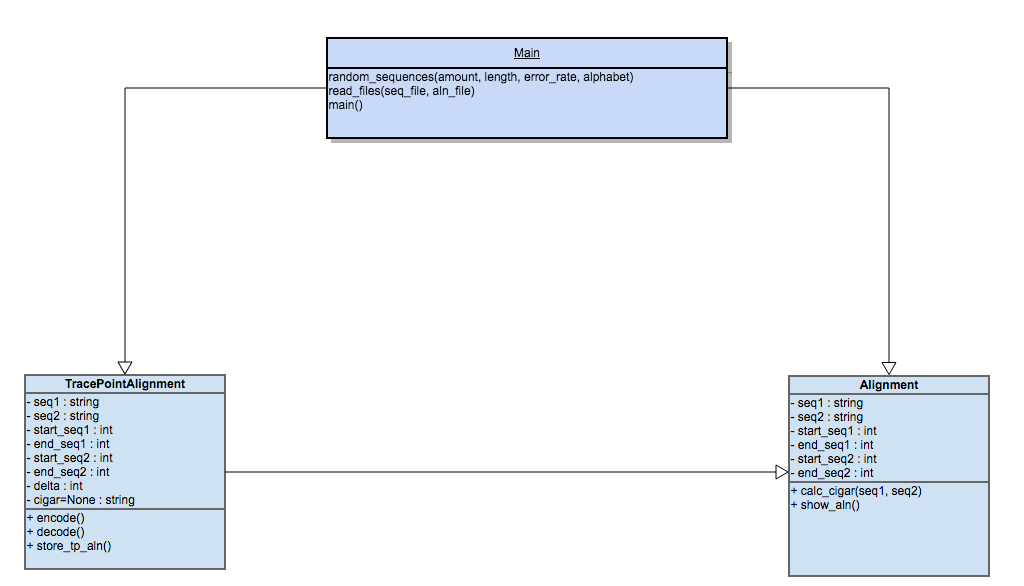
\includegraphics[width=\textwidth]{images/UML}
\section{Funktionalit�t}
\subsection{Informationsverlust bei 'encode()'}
Die encode-Funktion extrahiert aus dem gegebenen CIGAR-String die Trace Points, welche dann zusammen mit dem $\Delta$-Wert und den Start- und Endpositionen der Sequenzabschnitte gespeichert werden. Hierbei geht die Information, wie die jeweiligen Intervalle zwischen den Trace Points zu den komplement�ren Intervallen in der Ursprungssequenz aligniert werden, verloren.
F�r die R�ckgewinnung dieser Information muss in der 'decode()'-Funktion zun�chst ein neues Alignment der jeweiligen Intervall-Paare errechnet werden.

\section{Grafiken Geschwindigkeit, Speicher}



%
% Einleitung
%

\chapter{Fazit}


\cleardoublepage

% Anhang
%\appendix
%%
% Anhang
%

\chapter{Anhang}
Lorem ipsum dolor sit amet, consectetuer adipiscing elit. Cras semper. Integer sapien nulla, consectetuer a, laoreet et, varius quis, mauris. Nunc pharetra tincidunt massa. Pellentesque habitant morbi tristique senectus et netus et malesuada fames ac turpis egestas. Praesent pellentesque mauris at elit. Aliquam consequat suscipit enim. Pellentesque habitant morbi tristique senectus et netus et malesuada fames ac turpis egestas. Nunc sapien. Proin hendrerit diam at quam. Lorem ipsum dolor sit amet, consectetuer adipiscing elit. Integer vulputate semper nunc. Sed dui. Praesent at sem. Integer elit ipsum, placerat vitae, dictum quis, feugiat sit amet, metus.

\section{�berschrift zweiter Ordnung}
Donec arcu turpis, pretium quis, interdum non, condimentum a, est. Fusce lobortis urna non tellus. Nam leo dui, malesuada non, tempus placerat, congue eget, pede. Mauris porttitor risus quis tortor molestie vehicula. Curabitur tincidunt. In malesuada congue nisi. Nullam et nulla. Curabitur porttitor. Ut molestie sagittis felis. Sed urna libero, ultricies quis, laoreet eget, congue id, metus. Proin ac lorem cursus mauris auctor laoreet. Donec justo. Etiam nunc sem, dapibus sit amet, euismod a, molestie sit amet, mi.

Morbi sollicitudin consequat magna. Vivamus dictum. Nulla non quam. Nam sem tellus, aliquam sed, hendrerit nec, imperdiet ut, augue. Aliquam erat volutpat. Vivamus non ligula sit amet lorem accumsan viverra. Cras mattis libero et ante. Cras massa. Donec fringilla, metus vitae semper condimentum, dolor dui fringilla arcu, et mattis nulla dui vel lectus. Nunc mauris magna, tristique eu, rutrum at, facilisis eu, odio. Nullam congue magna non nisi. Suspendisse viverra, massa non pellentesque scelerisque, risus elit 

\noindent Hier kommt ein Listing \ref{lst:soap}.

\begin{center}
\begin{lstlisting}[caption={SOAP Anfrage an einen HalloWelt-Web-Service},label=lst:soap,language=XML,label={lst:soap}]
<?xml version='1.0' encoding='UTF-8'>
<SOAP-ENV:Envelope (*@\label{lst:soapEnv}@*)
  xmlns:SOAP-ENV="http://schemas.xmlsoap.org/soap/envelope/"
  xmlns:xsi="http://www.w3.org/2001/XMLSchema-instance"
  xmlns:xsd="http://www.w3.org/2001/XMLSchema"
  xmlns:ns1="http://localhost/wsdl/HalloWeltService.wsdl">
  
  <SOAP-ENV:Body>(*@\label{lst:soapBody}@*)
  	<ns1:gruss>
  		<name xsi:type="xsd:string">
  			Michael
  		</name>
  	</ns1:gruss>
  </SOAP-ENV:Body>

</SOAP-ENV:Envelope>
\end{lstlisting}
\end{center}

bibendum dolor, vitae ultrices lorem neque et erat. Nullam tortor ante, venenatis et, aliquet ac, ornare id, massa. Vivamus urna augue, posuere vitae, sagittis id, porttitor at, arcu. Praesent pharetra rutrum neque. Maecenas tempor ultrices felis.
Nulla facilisi. In sed elit aliquet neque malesuada blandit. Nam tempus imperdiet eros. Mauris tincidunt diam eu erat. Phasellus iaculis blandit leo. Nunc augue. Donec dignissim accumsan pede. Ut consequat, eros id accumsan placerat, mi justo ullamcorper pede, id lacinia augue nisi non nibh. Vestibulum eget arcu. Cras pretium, dui eu gravida varius, lectus neque accumsan ligula, eu sodales magna lectus ut nisi. Aliquam vel ante. Ut suscipit porta augue. Suspendisse pellentesque faucibus nisl. Nulla magna tortor, cursus quis, varius quis, hendrerit ut, neque.


%
% EOF
%
%\cleardoublepage

\phantomsection % ben�tigt f�r korrekte pdf-darstellung
\addcontentsline{toc}{chapter}{Literaturverzeichnis}
\bibliographystyle{natdin} % Din 1505 nach Lorenzen (Das konkrete Aussehen des Litverzeichnisses ist im header festgelegt)
\bibliography{bibliography/literatur}  % Pfad zur *.bib-Datei (Dateiendung wird weggelassen)
\cleardoublepage

\chapter*{Eidesstattliche Erkl�rung}
\thispagestyle{empty}
\addcontentsline{toc}{chapter}{Eidesstattliche Erkl�rung}

Ich versichere, dass ich die vorstehende Arbeit selbstst�ndig und ohne fremde Hilfe angefertigt und mich anderer als der im beigef�gten Verzeichnis angegebenen Hilfsmittel nicht bedient habe. Alle Stellen, die w�rtlich oder sinngem�� aus Ver�ffentlichungen entnommen wurden, sind als solche kenntlich gemacht. \\

%\noindent Ich bin mit einer Einstellung in den Bestand der Bibliothek des Fachbereiches einverstanden.

\vspace{2cm} 

\noindent Hamburg, den \uline{~~~~~~~~~~~~~~~~~~~~}~~~~~Unterschrift: \uline{~~~~~~~~~~~~~~~~~~~~~~~~~~~~~~~~~~~~~~~~~~~~~~~~~~} 


\end{document}
